\chapter{Preliminaries}

\begin{figure}
	\centering
	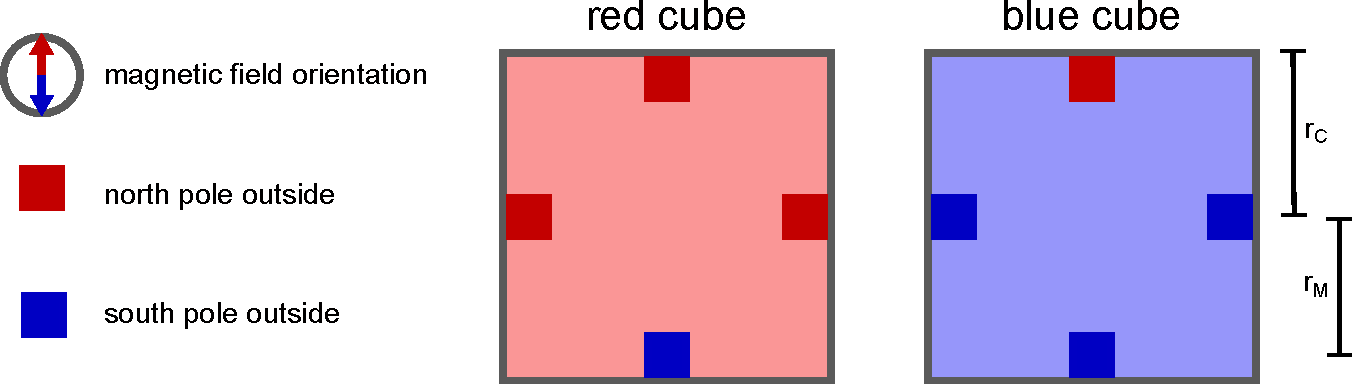
\includegraphics[width=0.90\textwidth]{figures/magnetic_cubes.pdf}
	\caption{Simplified top-down view of the two magnetic modular cube types with their outwards pointing magnet poles, illustrated as red and blue squares. Also visualizes the lengths $r_C$ and $r_M$}
	\label{fig:magnetic_cubes}
\end{figure}

\section{Magnetic Modular Cubes}
The magnetic modular cubes are cube shaped bodies embedded with permanent magnets on the four side faces.
The magnets have different orientations of their north and south pole. 
One pole is always pointing outside and the other straight to the center of the cube.
The magnet at the front face has its north pole pointing outwards and the magnet at the back its south pole.
These two magnets ensure, that the cube is always aligned with the global magnetic field and these orientations holds true for both cube types.
The two other side faces must have the same outwards pointing pole, so that its not possible for this axis to align with the magnetic field.
In fact this is the reason a distinct definition of front, back and side is even possible.
Since the front is always pointing to the north pole of the magnetic field, we also call it the north face, or north edge in two dimensions, and all the other faces can also be called by their corresponding cardinal direction.
For simplification we call magnets by their outwards pointing pole in further sections.
Furthermore two different cube types are defined:
Either both side magnets point out their north pole, these cubes are called red cubes, or they point out there south pole, which is called a blue cube.
Figure \ref{fig:magnetic_cubes} shows a top down view on the two cube types with all the outwards pointing magnet poles.
A compass always shows the orientation of the magnetic field in our illustrations.
Magnetic Modular cubes can be constructed in different sizes and ways. For more technical details and length measurements we refer to the original \cite{Bhattacharjee2022}.
Two important lengths that we use for planning and simulating, are the cube radius $r_C$ and the magnet radius $r_M$ (also illustrated in Figure \ref{fig:magnetic_cubes}).
$r_C$ is one half length of a cube face and $r_M$ is the distance from the center of the cube to the center of the magnet.

\section{Workspace And Configuration}

%the workspace only walls as obstacles, magnetic field abilities
%configuration. cubes at positions. Use graphic.
%Our configuration-space, SE(2)

\begin{figure}
	\centering
	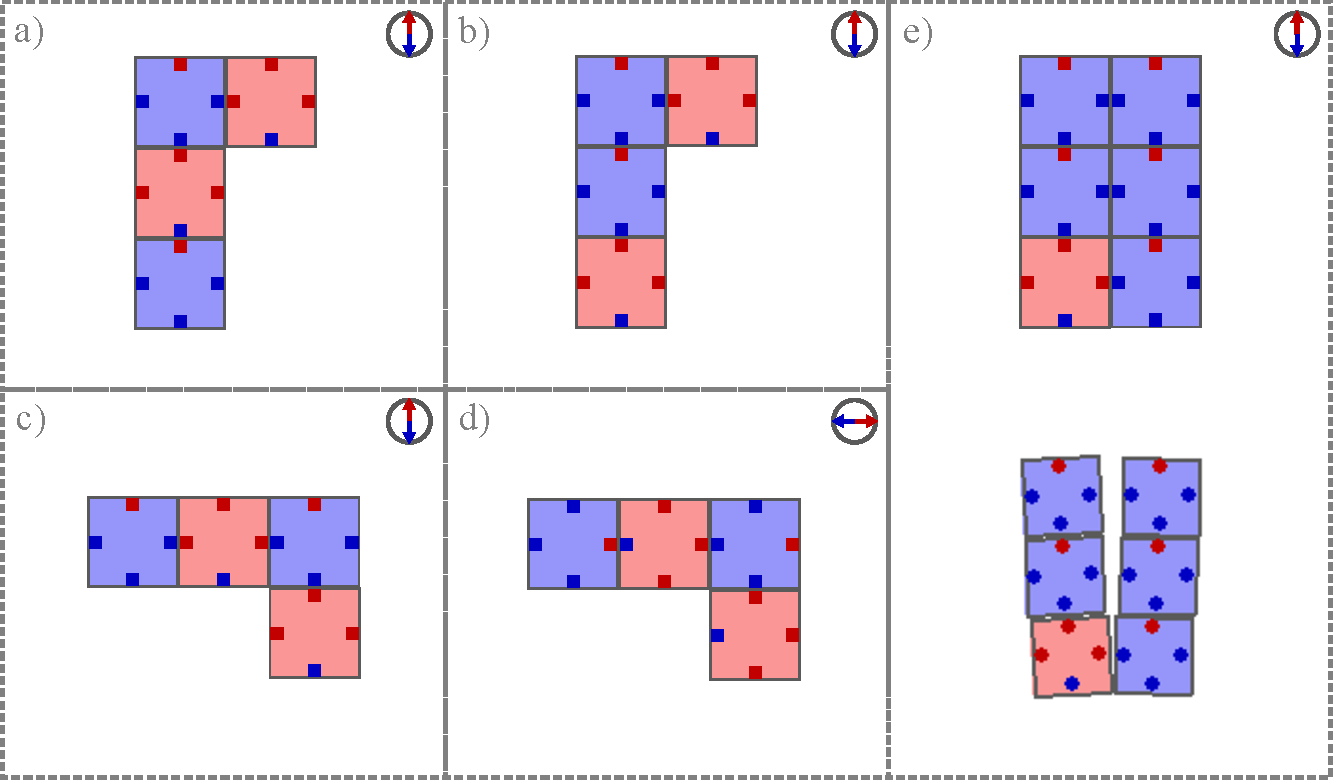
\includegraphics[width=0.90\textwidth]{figures/polyominoes.pdf}
	\caption{Polyominoes.}
	\label{fig:polyominoes}
\end{figure}

\section{Polyominoes}
%polyominoes. Fixed polys. Illegal polyominoes. Single cubes trivial polys, COM, pivot-foot/axis


\begin{figure}
	\centering
	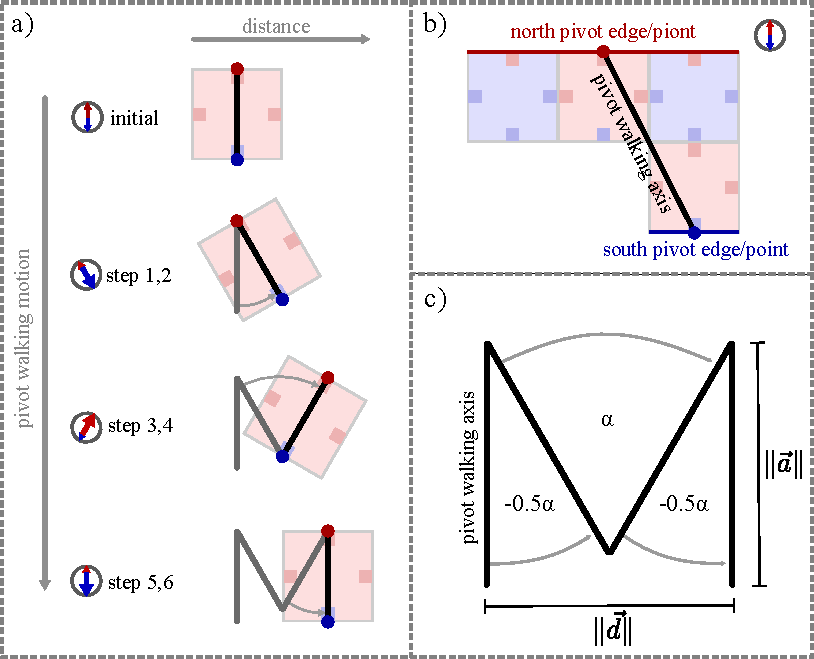
\includegraphics[width=0.80\textwidth]{figures/pivot_walking.pdf}
	\caption{pivot walking.}
	\label{fig:pivot_walking}
\end{figure}

\section{Motion}
%Rotation, Pivot-Walking, displacement for polys

